\documentclass[10pt]{article}
\usepackage[margin=.7in]{geometry}\usepackage{amsmath,amssymb,tikz,hyperref}
\setlength{\parindent}{0pt}\setlength{\parskip}{5pt}
\begin{document}
\textbf{Affine coefficient loop and bounded word arithmetic}\hfill2026-10-31\\T-1142. Producer proof packet; independent source-fidelity review pending.
\section*{Checked loop model}
For a field, input coefficients $c_k$ and scale $s$, define
\[R_k=\sum_{j=0}^{k}C\!\left(c_k\binom{k}{j}a^jb^{k-j}s^{-1}\right)X^j.\]
The row theorem proves $R_k=C(c_ks^{-1})(aX+b)^k$. Inner and outer prefix invariants then give, for arbitrary $n$,
\[\operatorname{outer}(n)=C(s^{-1})\left(\sum_{k<n}C(c_k)X^k\right)\!\circ(aX+b).\]
Slot updates affect only the selected coefficient. Removing a trailing zero preserves the represented polynomial. Taking $s=a^m$ connects this loop model to the preceding $T_m$ normalization theorem.
\begin{center}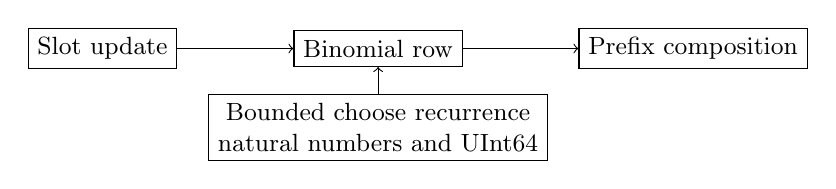
\begin{tikzpicture}[every node/.style={draw,align=center,font=\small}]
\node (a) at (0,0) {Slot update};\node (b) at (3.5,0) {Binomial row};\node (c) at (7.5,0) {Prefix composition};
\draw[->](a)--(b);\draw[->](b)--(c);
\node (d) at (3.5,-1) {Bounded choose recurrence\\natural numbers and UInt64};\draw[->](d)--(b);
\end{tikzpicture}\end{center}
\section*{Word bound and controls}
For every $0\le j\le k\le5$, the UInt64 recurrence equals$\binom{k}{j}$. Its pre-division products are at most 30, divisors are positive, and $30<2^{64}$. Index bounds give$j<n$, $j\le k$ and$k-j+j=k$ under the loop conditions. Degree 6 attains a product 60, so the 30 bound is deliberately limited to degree 5.

With $a=2,b=3,c=4,s=2$, rows 0/1/2 are $2$, $6+4X$, and$18+24X+8X^2$. The middle coefficient 24 rejects 12 from a missing binomial factor. Controls also cover zero/empty input, slot isolation, the final index, $\binom52=10$ and the attained 30 bound.
\section*{Evidence and source boundary}
Thirteen main declarations and fourteen controls have separate named axiom readback. Native exits and input hashes are checked. The main attempts passed with an unused-simp warning; the first control attempt failed on mapped rational constants, then passed after correction. Controls were rebuilt against the final word theorem.

The retained source excerpt and hashes bind \texttt{genus2\_model\_gate.rs}:1--56. Its inverse call requires $s\ne0$. Abstract totalized inverse at zero is not a source-execution claim. Prime-field encoding, \texttt{choose\%p}, field-operation correspondence, literal array/trim/compiler behavior and geometric class transport remain separate bindings. The word theorem concerns the bounded choose recurrence.

Sources: \href{https://leanprover-community.github.io/mathlib4_docs/Mathlib/Algebra/Polynomial/Taylor.html}{Mathlib Taylor}, \href{https://leanprover-community.github.io/mathlib4_docs/Mathlib/Algebra/Polynomial/Eval/Coeff.html}{evaluation/coefficient documentation}, and pinned \texttt{Data/Nat/Choose/Sum.lean}. No novelty claim. No scientific campaign, curve enumeration, timing or cost ratio. Diagram shows proof dependencies; cohort and campaign limits unchanged.
\end{document}
